\chapter{Einführende Flugtests: Misson-Mode}
Einführend wird die Verwendung von Bodenstation und Drohne im Missionsmodus beschrieben. Zum Einsatz kommt die Software \textit{QGroundcontrol} auf dem PC. 

\begin{multicols}{2}
    Der Missionsplaner kann jederzeit oben Links in \textit{QGroundcontrol}, wie in Bild \ref{fig:qgc_mission_plan} dargestellt, aufgerufen werden. Es öffnet sich ein erweitertes Menü. Nach dem Anlegen des jeweiligen Planes muss dieser zur Drohne hochgeladen werden (nur während eine Verbindung hergestellt ist). Anschließend kann der Missions-Planer verlassen und die jeweilige Mission über das wechseln in den Mission-Mode gestartet werden.
    \vfill\null
    \columnbreak
    \begin{figure}[H]
        \centering
        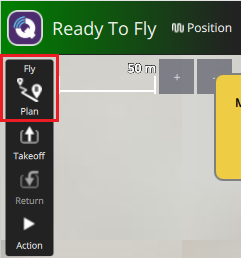
\includegraphics[width=0.4\textwidth]{images/mission_plan_open.png}
        \caption[QGroundControl Missionplaner-Menu]{QGroundControl Missionplaner-Menu wird durch Klick auf Rot umrahmten Button geöffnet}
        \label{fig:qgc_mission_plan}
    \end{figure}
\end{multicols}

\newpage
\section{Flug auf gerade Linie}
Für den einfachsten Fall lassen sich im Missionsplaner eine Liste von Wegpunkten anlegen, siehe dazu Bild \ref{fig:qgc_mission_plan_wp}. Nachdem am linken Rand \enquote{Waypoint} ausgewählt wurde lassen sich diese beliebig auf der Karte platzieren. Der erste Punkt beschreibt den Start, der letzte kann als Landepunkt dienen. Andernfalls kann die Drohne zum Startpunkt zurückkehren oder in letzter Position stehen bleiben.\\
Jeder Wegpunkt beschreibt eine Position im Raum. Die Parameter Höhe, Bewegungsgeschwindigkeit und eine relative Drehung zur Vorwärtsrichtung (Yaw) können für jeden Punkt separat am rechten Rand festgelegt werden.\\
Im unteren Bildbereich ist das Höhenprofil über den Weg eingezeichnet: in Orange gefärbt die jeweilige Flughöhe der Drohne, in Grün der Boden laut \gls{gps} Karte.\\
Mit den im Bild gezeigten Einstellungen wird die Drohne starten, auf gerade Linie nach vorn fliegen und anschließend landen. Dieses Verhalten wurde in der Simulation überprüft. Dazu wurde ein Hilfsprogramm geschrieben, welches die derzeitige Geschwindigkeit, Höhe und Orientierung der Drohne mitschreibt. Eine Auswertung als Diagramm ist zu sehen in Bild \ref{fig:qgc_mission_plan_wp_dia}.

\begin{figure}[h]
    \centering
    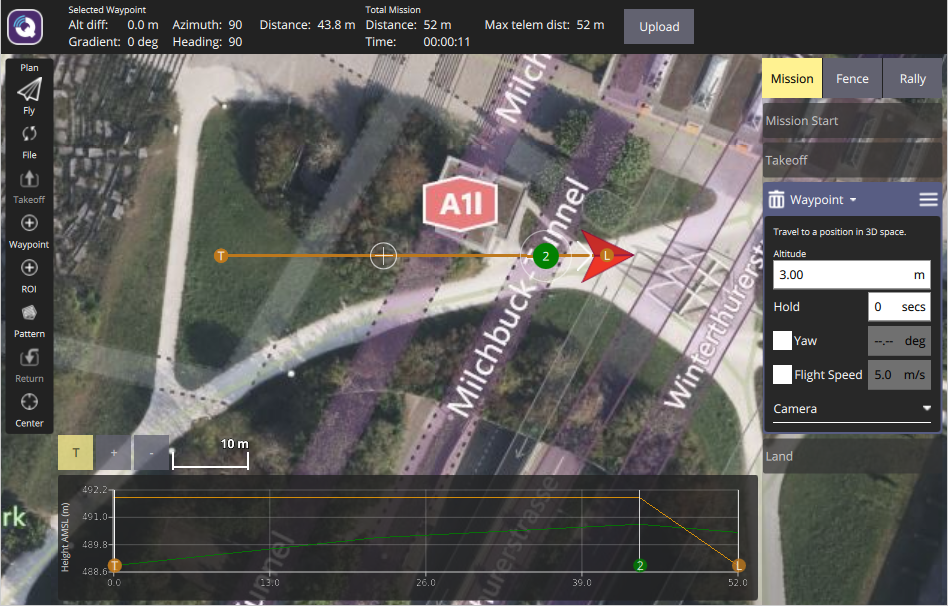
\includegraphics[width=0.6\textwidth]{images/mission_plan_mission.png}
    \caption[QGroundControl Missionplaner-Wegpunkte]{QGroundControl Missionplaner-Wegpunkte}
    \label{fig:qgc_mission_plan_wp}
\end{figure}

\begin{figure}[h]
    \centering
    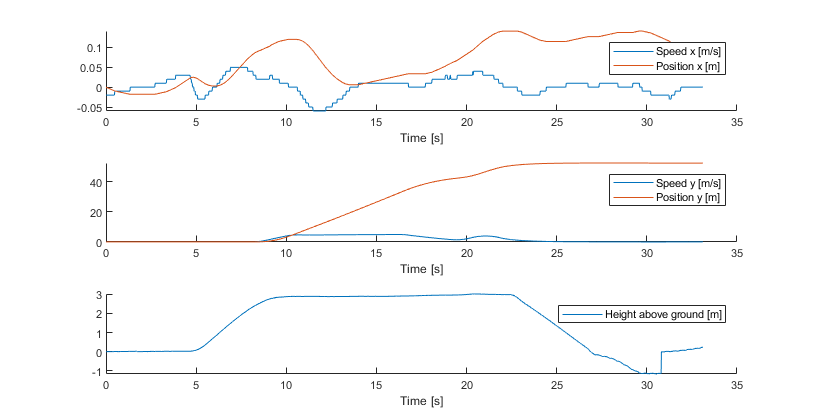
\includegraphics[width=0.9\textwidth]{images/mission_plan_mission_dia.png}
    \caption[Auswertung Missionsplaner-Wegpunkte]{Auswertung Missionsplaner-Wegpunkte: Diagramme geplottet von Matlab. In den oberen Diagrammen zu sehen sind die jeweilige x-/y-Geschwindigkeit und -Position während des Fluges. Positive x-Richtung zeigt nach Norden, positive y-Richtung nach Osten. Im unteren Diagramm die Flughöhe. Da der Simulator von einer flachen Welt ausging, die GPS-Karte aber eine Position in Östterreich annahm, wurde der Landepunkt höher als der eigentliche Boden angedacht. Durch verfrühtes Abschalten der Motoren "fiel" die Drohne auf den simulierten Boden, was zu Fehlern in der beschriebenen Höhe führte. Die Drohne konnte diesen Fehler beim Landen bei ca. $30s$ ausgleichen, hob erneut ab, um schließlich langsam zu sinken und blieb sicher stehen}
    \label{fig:qgc_mission_plan_wp_dia}
\end{figure}

\section{Rally-Punkte}
Neben den Wegpunkten können Rally-Punkte beliebig auf der Karte verteilt werden. Diese dienen als alternative Landepunkte. Wird während der Mission ein \enquote{Return to Land} ausgelöst (bspw. als letzter Punkt einer Mission, durch GeoFence, oder im Fehlerfall), fliegt die Drohne den nächsten Rally-Punkt an und landet. Das Verhalten ist in Bild \ref{fig:qgc_mission_plan_rp} dargestellt. Die Funktion kann zur Fehlervermeidung verwendet werden.

\begin{figure}[h]
    \centering
    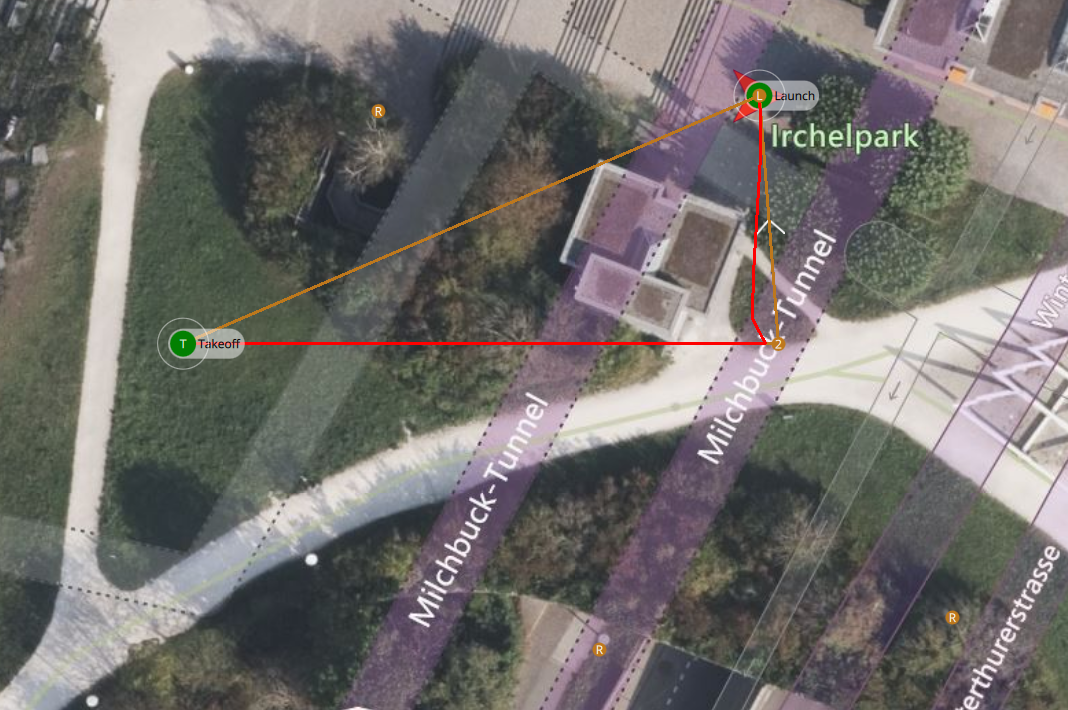
\includegraphics[width=0.6\textwidth]{images/mission_plan_rally.png}
    \caption[QGroundControl Missionplaner-Rallypunkte]{QGroundControl Missionplaner-Rallypunkte: 4 Rally-Punkte verteilt auf Karte um Flugbahn der Drohne. Nach Abschluss der Mission wurde der obere rechte Punkt angeflogen und gelandet}
    \label{fig:qgc_mission_plan_rp}
\end{figure}

\section{Flug mit Survey}
Anstatt Wegpunkte manuell anzulegen, können mit \enquote{Pattern}\footnote{siehe \url{https://docs.qgroundcontrol.com/master/en/PlanView/Pattern.html}} verschiedene Routen automatisch angelegt werden. Mit \enquote{Survey} kann ein Gebiet eingestellt werden, welches von der Drohne im überflogen wird. Im Auswahlmenü stehen verschiedene Formen wie Polygon oder Kreis zur Verfügung. Innerhalb dieser wird ein Zick-Zack Pfad aus mehreren Wegpunkten angelegt. Innerhalb des Konfigurationsmenü können Abstand und Winkel der Bahnen eingestellt werden. Die Drohne während der Abarbeitung einer Survey ist in Bild \ref{fig:qgc_mission_plan_surv} gezeigt. Neben Survey können noch weitere Planungsmodi \enquote{Corridor-Scan} und \enquote{Structure-Scan} angelegt werden. Bei ersterem fliegt die Drohne kontinuierlich eine gerade Strecke hin und her. Mit letzterem kann in verschiedenen Höhen um Objekte wie Gebäude geflogen werden, um Aufnahmen von der Beschaffenheit zu machen.

\begin{figure}[h]
    \centering
    \includegraphics[width=0.6\textwidth]{images/mission_plan_rally_scan.png}
    \caption[QGroundControl Missionplaner-Survey]{QGroundControl Missionplaner-Survey: Automatisch angelegte Wegpunkte werden angeflogen. Nach Start bei Punkt \enquote{T} flog die Drohne nach Norden zu Punkt \enquote{3} und befindet sich im Moment der Aufnahme in Drehung bei Punkt \enquote{9}}
    \label{fig:qgc_mission_plan_surv}
\end{figure}

\section{Flug mit GeoFence}
Ein GeoFence kann unabhängig einer Mission angelegt werden. Im Missionsmodus wird von \textit{QGroundControl}, vor Hochladen der Mission, überprüft, ob Punkte im betroffenen Beeich liegen. Trifft dies zu wird eine Fehlermedlung ausgegeben und das hochladen des Missionsplanes verhindert. Es gibt 2 Verhaltensmuster: Einschlüsse (die nicht Verlassen werden dürfen) und Ausschlüsse (die nicht Betreten werden dürfen).

Wird ein manueller Flug durchgeführt, kommt zuerst eine Warnung, dann stoppt die Drohne. Ein Beispiel für einen Einschluss ist in Bild \ref{fig:qgc_mission_geofence} gezeigt. Selbst bei mehrfachem Anflug war es nicht möglich die gekennzeichnete Zone zu erreichen. Die Drohne verfiel jeweils in den \textit{Hold}-Modus und musste zurückgestellt werden. 

\begin{figure}[h]
    \centering
    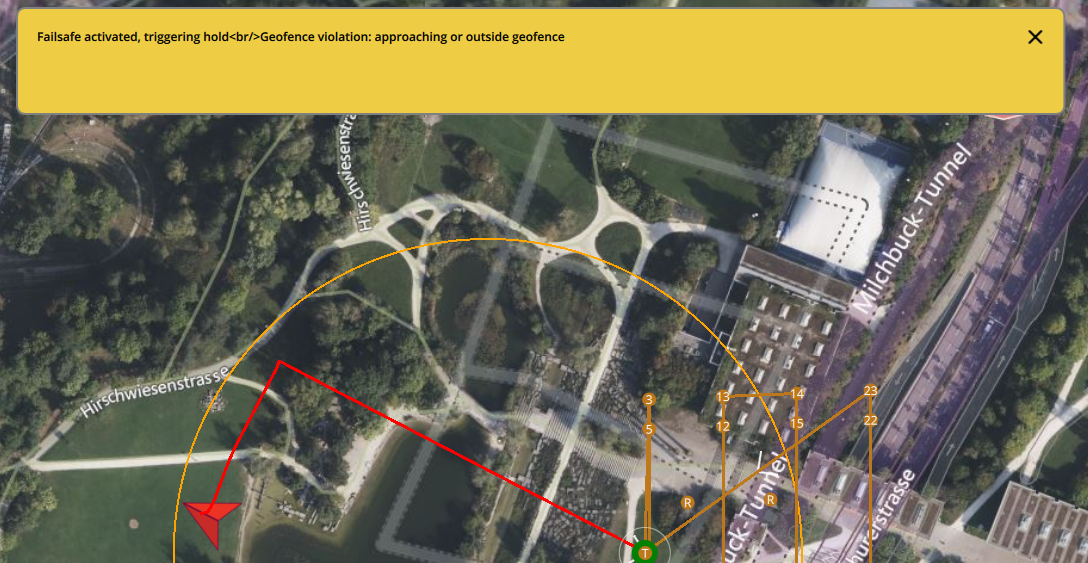
\includegraphics[width=0.6\textwidth]{images/mission_geofence.png}
    \caption[QGroundControl GeoFence]{QGroundControl GeoFence: Gelber Kreis stellt den GeoFence dar, den die Drohne nicht verlassen kann. Rote Linie zeigt den zurückgelegten Weg}
    \label{fig:qgc_mission_geofence}
\end{figure}

\section{Flug mit Region of Interest}
\glspl{roi} dienen der Orientierung der Drohne während einer Mission. Es können \glspl{roi}-Punkte gleich den Wegpunkten auf der Karte gesetzt werden. Um die Ausrichtung zu Verdeutlichen wurde Bild \ref{fig:qgc_mission_roi} aufgenommen. Es zeigt die Drohne als roten Pfeil, in Richtung des mit \enquote{R} markierten Punktes schauend. Ein Punkt ist solange gültig, bis er abgewählt oder ersetzt wird.

Das \gls{roi}-Kommando welches von \acrshort{mav} übertragen wird, kann später verwendet werden, um die Drohne gezielt auf Hindernisse zeigen zu lassen, falls diese sich außerhalb des Sichtbereiches der Sensoren aber noch innerhalb des Gefahrenbereiches der Drohne befinden.

\begin{figure}[h]
    \centering
    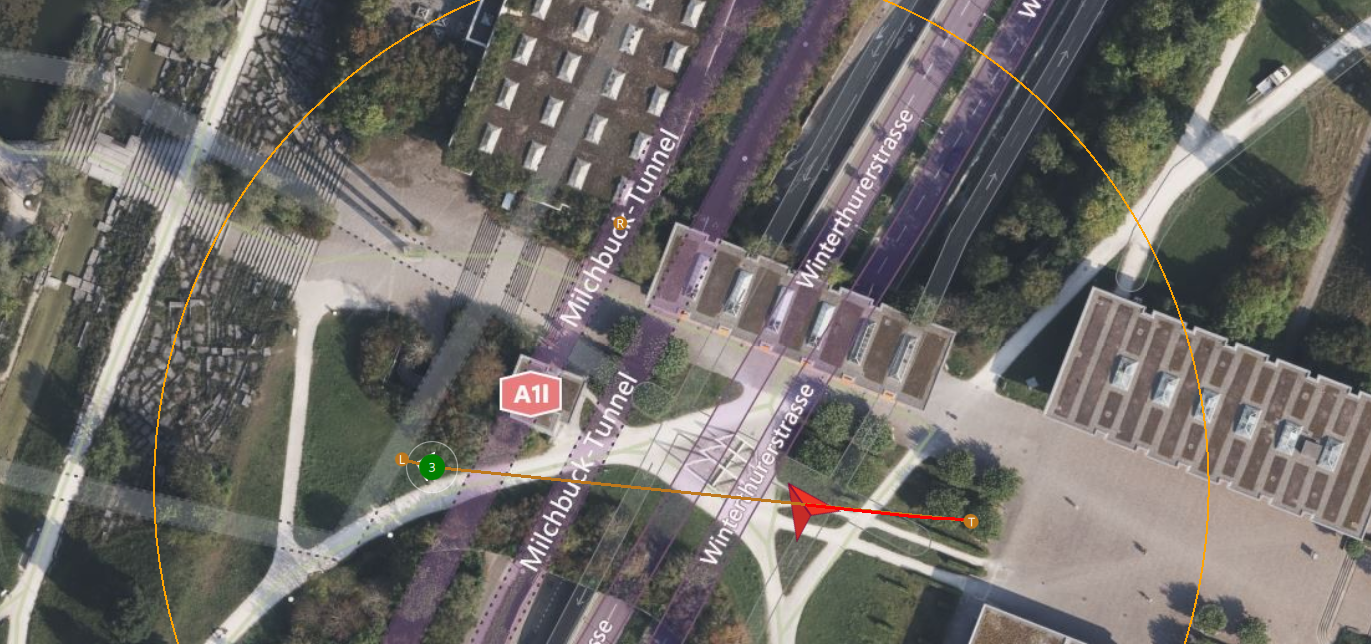
\includegraphics[width=0.6\textwidth]{images/mission_roi.png}
    \caption[QGroundControl Missionplaner-ROI]{QGroundControl Missionplaner-ROI: Während einer Mission zeigt die Drohne mit ihrem Bug in Richtung der mit \enquote{R} markierten ROI}
    \label{fig:qgc_mission_roi}
\end{figure}

\section{Zusammenfassung}
Für den angedachten autonomen Flugmodus eignet sich der Mission-Mode der Drohne nicht. Trotzdem sind Eigenheiten in der Flugsteuerung betrachtet wurden, die später wiederverwendet werden können. Ein Flug sollte grundsätzlich nur innerhalb eines GeoFence gestartet werden, um ein Entkommen der Drohne zu verhindern. Auch sind \acrshort{roi} hilfreich bei der Detektierung von Hindernissen. 
